\chapter{Analysis of the Attack against WBAES}
\label{chap:analysis}

%!% zase, viz preface
In this chapter we present some remarks of the attack introduced in Section \ref{sec:unify} against Klinec's implementation \cite{klinec2013implementation} of WBAES by Chow et al.\ \cite{chow2002aes}, denoted as {\tt KlinecWBAES}. Based on our observations, we suggest a blind attack (i.e.\ an attack without knowledge of the key) and mention some consequences in white-box design. % Then we outline why this attack is useful during white-box cipher design.
Finally we outline, justify and confirm an explanation of the attack.


\section{Blind Attack}
\label{sec:blindattack}

In a real-world scenario, the key is typically unknown. Therefore we do not have any information whether our best candidate is correct or not. We need some rule to recognize a fairly good candidate which we can obviously test for correctness by running AES encryption ourselves.

\begin{remark}
\label{rem:false}
	Especially note the attack against the \nth{1} byte using {\tt 3d} as a target and its last but one entry in Table \ref{tab:lintargets} -- here the incorrect candidate has a gap of almost $26\%$. It is actually the largest gap of an incorrect candidate among all targets and all bytes using this particular instance of WBAES tables. The largest gap of an incorrect candidate ever seen was almost $35\%$!
	%!% až prohodim pořadí v tabulkach tak i tady v tůtom remarku
	In our results, the target bits keep their original order (but reverse), therefore we can deduce the vector $B$ generating the target in terms of $T_B$. Here it is the second row of matrix of multiplication by $\texttt{3d}\pmod{x^8+1}$, see Example \ref{ex:shiftmatrix}. Hence the vector is $B = 01011110$.
\end{remark}

In order to perform a blind attack, we studied our results deeper, in particular we are interested in success rate of individual targets. The following section gives some of our remarks, next we suggest the blind attack itself in Section \ref{sec:subblindattack}


% ==============================================================================
% ===   R E M A R K S                                                        ===
% ==============================================================================

\subsection{Remarks}
\label{sec:remarks}

%~ We decided to create another {\tt KlinecWBAES} table instantiations in order to have larger data set. Note that for each instance we have $16$ independent tables -- one for each byte since %?% neni to podle mě uplně nezávislý ptž MC je před MB tže dycky aspon 4 byty jsou provázaný
We cannot make conclusions based on a single {\tt KlinecWBAES} table instantiation only. In order to avoid specific behavior of a single instance, we created another $7$ instances. Then we acquired $1024$ traces and ran attack against each of $16$ key bytes using all $255$ targets, for each instance. Altogether we ran $16\cdot255\cdot8=32\,640$ attacks which, together with trace acquisition and filtering, took us several hours on a regular hardware.

We processed the results and displayed several statistics, here we present some of them. Note that we only considered strong candidates as introduced in Note \ref{note:strong} (candidates with a gap greater than $10\%$).

The good news is that the overal success rate was $25\%$ (compare to $27\%$ and $31\%$ for our previous single-instance attack using the original SBox and Rijndael inverse, respectively) which gives us a hope that the new targets are successful as well. But our goal is rather to estimate individual success rate of each of our $255$ targets. (Another good news is that each target was successful at least once out of $16\cdot8=128$ chances.)

\subsubsection{Success Rate of Individual Targets}
	
	Remind that we have $255$ targets and only $8$ independent instances of tables which is quite a small data set for statistical purposes. For this reason, we rather group targets by different criteria and observe if they appear to be uniformly distributed. Note that this way we could possibly only refute uniformity, but it can still serve as reasonable justification.
	
	\paragraph{Group by corresponding $p$.}
	
	%~ We studied whether there is some influence of target invertibility (non-invertible targets were introduced in Section \ref{sec:noninv}).
	
	Here we make use of our former approach and group the targets by the corresponding $p$, see the transfer in Section \ref{sec:unify}. We put the results in a histogram, see Figure \ref{fig:leaktargethist}. Here we give percentual success rate for each group of targets together with their standard deviation (among $8$ measurements). Originally invertible $p$'s are in green, non-invertible in orange.
	
	\begin{figure}[h]
	\begin{center}
		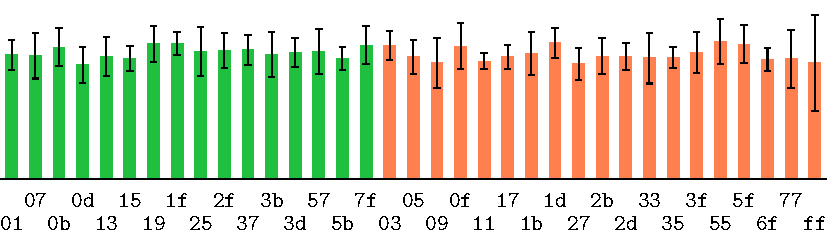
\includegraphics{figures/leak_target/leak_target.pdf}
		\caption{Success rate by targets' corresponding $p$'s and their standard deviation. Green represents invertible $p$'s, orange noninvertible ones.}
		\label{fig:leaktargethist}
	\end{center}
	\end{figure}
	
	%~ Note high deviation at {\tt ff}, this is because there is only a single target in this group (one generated by $B^T = (1,1,1,1,1,1,1,1)$).   %!% totál blbost, dev se přece nemůže zlepšovat počtem měření ne?
	Note that we did not give $y$-axis scale since the purpose is only to distinguish uniform distribution.
	
	\paragraph{Group with fixed $4$ bits in $B$.}
	
	Another way of grouping we performed, groups targets by fixing $4$ out of $8$ bits of their corresponding vector $B$, see Equation \ref{eq:tba}. We fixed the first and the last $4$ bits and grouped them, see results in Figure \ref{fig:leaktargetotherhist}, where these ways of grouping are in green or orange, respectively. Group index can be computed as binary AND of mask {\tt 0xf0} or {\tt 0x0f} with vector $B$, respectively.
	
	\begin{figure}[h]
	\begin{center}
		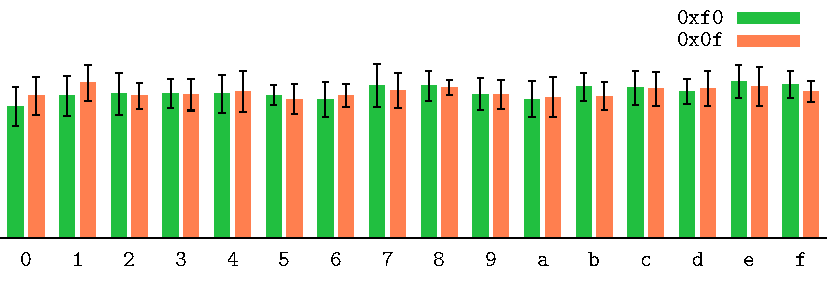
\includegraphics{figures/leak_target_other/leak_0x0f_0xf0.pdf}
		\caption{Success rate by fixed $4$ bits of targets' corresponding vector $B$. Green represents fixed first $4$ bits, orange represents last $4$ bits.}
		\label{fig:leaktargetotherhist}
	\end{center}
	\end{figure}
	
	\begin{remark}
	\label{rem:uniform}
		According to our observations, there does not seem to be a preferred target or a group of targets, therefore we will assume that target success rate is constant across all targets.
	\end{remark}

\subsubsection{False Positives}
	
	There is an inconvenience which emerges once we do not know the key -- we do not recognize the correct candidate anymore (see Remark \ref{rem:false}). Therefore we observed behavior of the incorrect ones.
	
	\paragraph{Gaps of incorrect candidates.}
		
		Previously we defined a strong candidate as a candidate with a gap larger than $10\%$. Most candidates which exceeded this limit were also correct candidates, but there were a couple of exceptions which we will refer to as {\em false positives}. Note that $25\%$ of candidates were strong and correct, on the other hand, there were $11\%$ of strong and incorrect ones. On average, strong incorrect candidates had a gap of $14\%$ (cf.\ $40\%$ for correct ones) and the highest gap ever seen was $35\%$ (cf.\ $76\%$ for correct ones). We need another observation about incorrect candidates in order to distinguish them from the correct ones.
		% 1024:
		% strong & correct:
		% 	[1019, 1000, 978, 1008, 986, 1006, 1019, 999] => 1001.875 ... 24.6%
		% 	[39.46, 39.68, 39.5, 40.28, 40.2, 39.85, 39.86, 39.68] => 39.81375
		% strong & incorrect:
		% 	[442, 440, 425, 415, 433, 463, 413, 468] => 437.375 ... 10.7%
		% 	[14.05, 14.06, 14.16, 13.95, 14.26, 13.83, 14.0, 13.97] => 14.035
	
	\paragraph{Number of repetitions of strong incorrect candidates.}
		
		The good news is that incorrect candidates do not repeat among targets very often. We observed the number of most repeating strong incorrect candidates among our $255$ targets and got following results: on average, the number was $1.75$, the maximum was $3$.
		% 	[1.88, 1.75, 1.81, 1.81, 1.62, 1.88, 1.62, 1.62]

\subsubsection{Using Less Traces}
	
	So far we used $1024$ traces in our attack, let us have a look at results of the attack with much less traces. Note that Bos et al.\ \cite{bos2015differential} used $2000$ and $500$ traces for the attack targetting the original SBox and Rijndael inverse, respectively.
	
	We used also much less traces, namely $128$, $256$, $384$ and $512$. For each number of traces we attacked all of our $8$ instances of {\tt KlinecWBAES} and observed success rate of strong candidates and their average gap. See results in Table \ref{tab:ntraces}.
	
	\begin{table}[h]
		\begin{center}
		\begin{tabular}{| c | c | c | c | c | c | c | c |}
			\hline
			Traces       &    $128$ &    $256$ &    $384$ &   $512$ &   $1024$ \\
			\hline
			Success rate &  $9.8\%$ &   $17\%$ &  ?       & ?       &   $25\%$ \\
			\hline
			Average gap  &   $24\%$ &   $32\%$ &  ?       & ?       &   $40\%$ \\
			\hline
			Reduced cost\footnote{Will be introduced later.}
			             & $5\,400$ & $4\,700$ & $.$ & $.$ & $10\,500$ \\
			\hline
		\end{tabular}
		\end{center}
	\caption{Success rates and average gaps using different numbers of traces.}
	\label{tab:ntraces}
	\end{table}
	
	% 128:
	% strong & correct:
	% 	[388, 420, 391, 411, 402, 393, 412, 397] => 401.750 ... 9.8%
	% 	[24.23, 24.39, 24.26, 23.65, 24.5, 24.01, 23.87, 23.65] => 24.07
	% strong & incorrect:
	% 	[262, 325, 351, 322, 309, 342, 285, 315] => 313.875 ... 7.7%
	% 	[13.34, 13.34, 13.13, 13.12, 12.9, 13.22, 13.26, 13.33] => 13.205
	
	% 256:
	% strong & correct:
	% 	[700, 670, 658, 722, 700, 709, 707, 683] => 693.625 ... 17.0%
	% 	[31.74, 32.49, 32.41, 31.83, 32.29, 31.31, 31.91, 32.11] => 32.01125
	% strong & incorrect:
	% 	[431, 472, 423, 441, 447, 451, 424, 482] => 446.375 ... 10.9%
	% 	[13.82, 13.85, 13.69, 14.1, 14.01, 14.1, 13.95, 14.36] => 13.985
	
	% 384:
	% strong & correct:
	% 	[814,791,784,825,790,819,812,]
	% 	[35.84,35.59,35.14,35.26,36.19,35.26,35.77,]
	% strong & incorrect:
	% 	[491,488,484,504,487,464,509,]
	% 	[14.17,14.37,13.97,14.17,14.14,14.07,14.23,]
	
	% 512:
	% strong & correct:
	% 	[879,851,855,887,848,]
	% 	[37.25,37.47,36.58,37.66,38.04,]
	% strong & incorrect:
	% 	[471,480,473,478,472,]
	% 	[14.02,14.09,13.96,13.97,14.23,]

\subsubsection{Leaking Bits}
	
	Remind that our trace is a bit-wise serialization of least significant bytes of memory addresses, hence we can identify which bit within that byte leaked -- simply by taking the leaking position within trace modulo $8$. This moduled position will be referred to as {\em leaking bit} (note the difference from target bit).
	
	We noticed soon that leaking bits are not very well balanced (as one would expect), therefore we put this data into a histogram, see Figure \ref{fig:leakbitall}. The histogram shows the amount of correct candidates with a gap larger than $10\%$ averaged over $8$ WBAES instances, for each leaking bit, together with standard deviation which is surprisingly very low. Note that the histogram does not provide absolute values since these could be misleading, only distribution is relevant at the moment.
	
	\begin{figure}[h]
	\begin{center}
		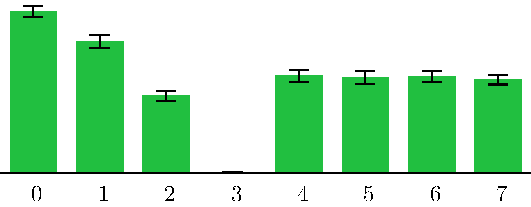
\includegraphics{figures/leak_bit/leak_bit.pdf}
		\caption{Average number of leaks and its standard deviation at each bit within trace.}
		\label{fig:leakbitall}
	\end{center}
	\end{figure}
	
	The \nth{0} and \nth{1} bits leaked slightly more, the \nth{2} bit slightly less and the \nth{3} bit actually leaked only twice while the overal average of the remaining bits was almost $160$! On the other hand, all of the remaining bits leaked fairly similarly. We do not have any explanation for this behavior.


% ==============================================================================
% ===   B L I N D   A T T A C K   S U G G E S T I O N                        ===
% ==============================================================================

\subsection{Blind Attack Suggestion}
\label{sec:subblindattack}

\begin{note}
	This section only applies previous observations on a heuristic basis, there is no guarantee that our approach is the best.
\end{note}

In general, we suggest to use rather less traces and repeat the attack with several targets until the sum of strong gaps of any candidate exceeds given bound.

According to results in Table \ref{tab:ntraces}, we attempt to estimate convenient number of traces. For this reason, we introduce {\em reduced cost of gap}, defined as
\begin{equation}
\label{eq:redcost}
	C(n, s, g) = \frac{n}{s\cdot g} ,
\end{equation}
where $n$ stands for the number of traces, $s$ for average success rate and $g$ for average gap of a strong candidate. Note that this quantity corresponds with average time of the attack: the more traces, the longer time; the better success rate or the bigger gap, the shorter time. Thus we can use this measure to compare expected time of the attack using different number of traces.


% omitting strong candidates' bound leads to ~1.5\% enhancement

% We rather suggest the following:
%~ \begin{enumerate}
	%~ \item pick a target, %?% Chi-square test of uniformity, pick random
	%~ \item attack using $256$ traces
%~ \end{enumerate}
% 10\% pro započtení, 75\% kumulativní mez? moc často se totiž neopakujou
% vyzkoušet jestli tak zlomim všechny instance

%~ Therefore, in case of blind attack (i.e.\ no knowledge of actual key), we suggest to use less traces, but keep changing the target until the maximal gap exceeds $27\%$, then we accept that candidate. This is likely to happen soon since $10.6$ out of $16$ targets succeed on average.

% psal já / Teuwen:
%~ > I only wonder about the reasoning why Karroumi is more than Chow since
%~ > it seems to have been shown to be equal (based on what I wrote in my
%~ > previous email).
%~ 
%~ Well I've no problem to break completely Chow with standard DCA so there
%~ is something a bit more in Karroumi. Obviously not enough to make it
%~ robust enough...


\section{Use in White-Box Cryptography Design}
\label{sec:useindesign}

The benefit of this attack is obvious -- it introduces a principially different approach to break white-box cryptography implementations. This attack may help to address weaknesses of any future white-box cryptography implementation and possibly increase its resistance to this kind of attack.

So far, we were only interested in results of the attack. In this section, we will study practical consequences of the attack itself. First we describe our initial effort trying to identify which intermediate product causes the leakage, then we outline some countermeasures against this attack. Both might be useful in white-box cryptography design.


% ==============================================================================
% ===   P O I N T   O F   L E A K A G E                                      ===
% ==============================================================================

\subsection{Point of Leakage}
\label{sec:leakpoint}

Note that the attack allows us to reveal concrete addresses which contributed to the key recovery. Our original intention was to find the corresponding piece of source code, and possibly deduce the intermediate product, which is later transformed into leaking memory address, -- it would most likely be used as an array index.

We tried two ways of using a debugger how to find that position in source code, but neither of them gave any results. Authors of the DCA toolkit \cite{bos2016tools} were successful at this point, see their comprehensive and very technical report on a wiki page of their Deadpool repository\footnote{Direct link:\\\link{github.com/SideChannelMarvels/Deadpool/wiki/Tutorial-\%234\%3A-DCA-against-Karroumi-2010-challenge}.\\Accessed 2016-04-24.}.

One could possibly try yet another approach -- modify the source code to output directly all relevant array indexes. Note that it might be challenging to address them really all.

However, we did not finally make use of this information (i.e., the point of leakage in source code) -- we identified the leaking intermediate product rather by a mathematical reasoning. This will be given in Section~\ref{sec:attempt}.

% LEGACY !!!
% BEGIN
%~ \begin{description}
	%~ \item[Watchpoint in GDB.]
		%~ We acquired one full trace (as described in Section~\ref{sec:filter} under the caption ``\nameref{subsec:atf}'') for some plaintext used during the acquisition phase. We checked that this trace perfectly matches the corresponding trace from the acquisition phase.
		%~ 
		%~ We identified the leaking address and set up a watchpoint in GDB running in the same terminal session. However, GDB did not catch the address, probably because PIN uses different virtual environment.
	%~ \item[GDB connected to PIN's debugging interface.]
		%~ We set up a connection between PIN application debugging interface and GDB as described in PIN manual \cite{pin214manual}, but could not catch {\em any} address. GDB was complaining that it cannot insert hardware breakpoint, on the other hand, software breakpoints did not work either.
	%~ \item[Outputting all array indexes.]
		%~ Note that array indexes are very likely the values which are later transformed into leaking memory addresses. Hence it should be possible to output and attack all indexes used within the encryption procedure. However we did not succeed with the first attempt -- it required certain reasoning and finding the specific intermediate result to output; both will be given in Section~\ref{sec:attempt}.
%~ \end{description}
% END


% ==============================================================================
% ===   C O U N T E R M E A S U R E S   A G A I N S T   D C A                ===
% ==============================================================================

\subsection{Countermeasures against DCA}

Since DCA is based on an algorithm, which was originally developed for physical measurements of certain hardware emissions, we can look for some inspiration back in hardware model. There are several countermeasures, see the following list for some of them (basic ones are introduced in \cite{chari1999towards,goubin1999des}).
\begin{description}
	\item[Masking with random values.] Cryptographic hardware can run some unpretendable source of random data and thus mess up values in traces (i.e., adding a strong noise). However, there is no equivalent of noise in white-box context, since everything is is fully controlled by the attacker.
	\item[Reordering instructions.] Remind that our algorithms required aligned traces, therefore it would be fatal if the leaking position were at several different places. However, this could be possibly overcome in white-box context -- we could achieve this by reverse engineering or, much easier, by aligning the traces with respect to instruction address trace (as outlined by Bos et al.).
	\item[Adding random delays.] Note that random delays have very similar properties as the previous countermeasures -- it can be controlled by the attacker and it only causes a trace misalignment.
\end{description}
In general, we cannot rely on any source of {\em dynamic} random data (generated during program execution). All we need to rely on is {\em static} random data (generated during instantiation). On the other hand, dynamic randomness can be used in a white-box implementation -- just as another level of ``obfuscation''.

Bos et al.\ further propose to use some ideas from {\em threshold implementations} \cite{nikova2006threshold} or use of external encodings -- here they emphasize that more research is needed.


\section{Explanation Attempt}
\label{sec:attempt}

First of all, let us remind the information flow through WBAES tables (originally in Equation \ref{eq:wbaesflow}), especially its first table.
\begin{equation}
\label{eq:wbaesfirst}
	\ldots \rarr \underbracket{\Enc \rarr \IMB^{-1} \xrightarrow{\textnormal{plain}} \TBox \xrightarrow{\textnormal{plain}} \MB \circ \MC \rarr \Enc^{-1}}_{\textnormal{in table}} \rarr \ldots
\end{equation}
Note that the last plain AES state (denoted with ``plain'' in the previous equation) is actually an $8$-bit output of the first SBox i.e.\ the very original target. Let us see what happens next: a composed linear mapping $\MB\circ\MC$ is applied resulting in a $32$-bit output (using an idea outlined in Section \ref{sec:aeslookup}), then each $4$-bit nibble is passed through a $4$-bit random bijection $\Enc^{-1}$ (further simply $\Enc$).

\begin{description}
	\item[$\MB\circ\MC$.] We can view each bit $t$ of the $32$-bit output of $\MB\circ\MC$ as a scalar product of a row $[R]^T$ of matrix representing $\MB\circ\MC$ (i.e.\ a random-like\footnote{Cannot be zero (follows from Note \ref{note:fullrank}).} $8$-bit vector) with its $8$-bit input $[S]$ which is actually an output of the first SBox. We get
	\begin{equation}
		t = [R]^T\cdot [S] = [R]^T\cdot\Bigl( \{\texttt{1f}\}\cdot\bigl([K]+[P]\bigr)' + [\texttt{63}] \Bigr) ,
	\end{equation}
	where $\{\cdot\}$ stands for respective binary matrix of multiplication modulo $x^8+1$ and $(\cdot)'$ for Rijndael inverse (i.e.\ there is the output of the first SBox in the big parantheses, cf.\ Equation \ref{eq:sbox}). This equation can be easily turned into the form of previously used target (Equation \ref{eq:tba}), indeed
	\begin{align*}
		[R]^T\cdot\Bigl( \{\texttt{1f}\}\cdot\bigl([K]+[P]\bigr)' + [\texttt{63}] \Bigr) &= \bigl([R]^T\cdot \{\texttt{1f}\}\bigr)\cdot\bigl([K]+[P]\bigr)' + \bigl([R]^T\cdot [\texttt{63}]\bigr) = \\
		&= [\bar R]^T \cdot \bigl([K]+[P]\bigr)' + \bar r ,
	\end{align*}
	where $\bar R$ is just a different random-like vector, which plays the role of $B$ in Equation \ref{eq:tba}, and $\bar r$ is a constant bit. Remind that additive constant does not need to be considered inside target (see Remark \ref{rem:pqeffect}). It follows that each of these $32$ bits perfectly matches some of our $255$ targets introduced in Section \ref{sec:unify}.
	
	%!% nebylo tu, zakamuflovat
	Note that, even though $\MB\circ\MC$ introduces diffusion, there is no diffusion so far, because those $32$-bit intermediate results are not combined together so far. Therefore these intermediate results only depend on single input byte!
	
	If we could observe these intermediate results, we would get the difference of means equal to $1.0$ (cf.\ attack against unprotected implementation in Section \ref{sec:naiveaes}).
\end{description}
\begin{remark}
\label{rem:enc}
	It follows that the protection against our $255$ targets is fully and solely accomplished by $\Enc$.
\end{remark}
\begin{description}
	\item[$\Enc$.] Remind that $\Enc$ is a (only) $4$-bit random bijection. Note that, unlike confusion elements in regular ciphers (e.g.\ SBox in AES), there is no nonlinearity check\footnote{Linearity in ciphers is studied by {\em linear cryptanalysis}, see e.g.\ \cite{matsui1993linear} for detail.} in WBAES by Chow et al.\ \cite{chow2002aes}.
	
	The choice of $\Enc$ actually only relies on the fact that the ratio of affine mappings among all random bijections is extremely low (less than $0.000\,002\%$ for $4$-bit bijections). This justification is very poor since it does not even address the case where only one output bit of $\Enc$ is an affine mapping of the input!
	
	There are actually quite many bijections which are affine in single output bit. Indeed, there are $2\cdot4\cdot(2^4-1)\cdot8!\cdot8! \approx 2\cdot10^{11}$ of them among $16! \approx 2\cdot10^{13}$ bijections on $4$-bits altogether which already makes some $1\%$ ratio! Also note that in such case, the maximum difference of means would be still $1.0$ since this affine mapping could be composed with the previous affine mappings yielding an affine mapping again.
	
	But we do not necessarily need a fully affine mapping at some bit, it would be sufficient if the mapping were affine for most inputs. Clearly, there are much more such mappings. For this reason, this intermediate result of WBAES seems to be most likely that which causes the leakage.
\end{description}

To support our hypothesis, we modified the source code of {\tt KlinecWBAES} to output these intermediate products (i.e.\ outputs of the first Type II tables, see Equation \ref{eq:wbaesflow}) and ran the attack with these values instead of memory traces. The attack indeed succeeded, which fully supports our explanation.

However, we noticed an interesting thing: leaking bits, as introduced in Note \ref{note:leakbit}, appear to be uniform in this case!

% perla (jakože fakt nebrat vážně): Note that a random bijection is extremely unlikely to provide any correlation between any input and output bit.


